\documentclass[a4paper,10pt]{report}
\usepackage[utf8]{inputenc}
\usepackage{graphicx} 

% Title Page
\begin{document}

\begin{titlepage}
    \centering
        {\bfseries\Large
        Kaggle Titanic competition\\
        March 2015
        
    }  
     \vfill
     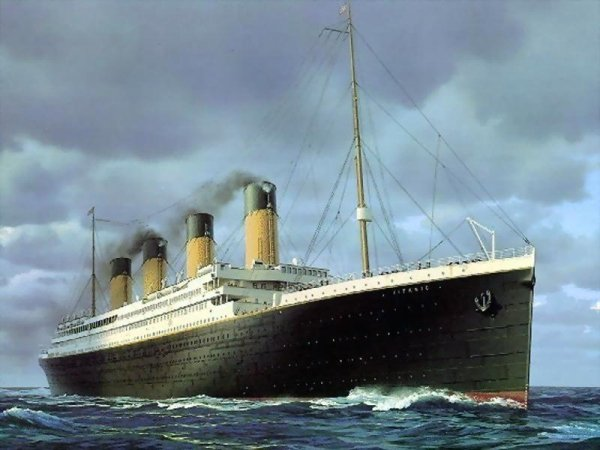
\includegraphics[width=10cm]{titanic.jpg} % also works with logo.pdf
    \vfill
    {\bfseries\Large

        Nicolas Legroux - Hugo Braun\\
        \vskip2cm
        INF582
    }    
    \vfill
   
  
\end{titlepage}

\section*{Introduction}
The Titanic Kaggle competition defines a data science challenge : By using a few features on the passengers onboard
(Name, Age, Family characteristics...) and a train dataset, we have to predict if a passenger has died during the sinking. 
To solve the problem, we tried different approaches, by using various classifiers and performing features engineering,
which lead us to a final score of 0.82297

\section{Input data}
\subsection{Structure}
The input data is separated in two parts : the train data, which contains the 'survived' information, and the test data
on which we have to apply our prediction algorithm.
The data contains the following values :
\begin{enumerate}
 \item PassengerId 
 \item Pclass : the passenger's class in the ship
 \item Name : Contains many informations, like the Surname, the Title (Mr., Mrs., etc...) and the maiden name for a married woman
 \item Sex
 \item Age 
 \item SibSp : Number of siblings aboard
 \item Parch : Number of parents/children aboard
 \item Ticket : String that describes the ticket number
 \item Fare : Price paid for the ticket (a ticket can be shared)
 \item Cabin
 \item Embarked : Port where the passenger embarked
\end{enumerate}

Some features were missing values. The first step was to prepare the data

\subsection{Preparing the data}



\end{document}          
